\section{Proof Refactoring and Repair}
\label{sec:overview}

\begin{figure}
\begin{minipage}{0.46\textwidth}
   \lstinputlisting[firstline=1, lastline=3]{listswap.tex}
\end{minipage}
\hfill
\begin{minipage}{0.46\textwidth}
   \lstinputlisting[firstline=5, lastline=7]{listswap.tex}
\end{minipage}
\caption{The updated \lstinline{list} (right) is the old \lstinline{list} (left) with its two constructors swapped (\codediff{orange}).}
\label{fig:listswap}
\end{figure}

\toolname is a tool for proof refactoring and repair that is available on Github.\footnote{Link withheld for double-blind review.}
Proof refactoring and proof repair are similar problems: both refer to adapting proofs in response to changes
in specifications. Refactoring refers to semantics-preserving changes, and repair refers to non-semantics-preserving
changes. In both cases, we can think of \toolname as \textit{reusing} the old proof about some old specification
to derive a proof about some new specification.

Consider a simple example: refactoring list proofs after swapping the two constructors of a list (Figure~\ref{fig:listswap}).
Even such a simple change can quickly cause trouble in existing proofs, like this proof from the Coq standard library:\footnote{Here and throughout, we use induction instead of pattern matching.}

\begin{lstlisting}
Lemma rev_app_distr {A : Type} :
  forall (x y : list A), rev (x ++ y) = rev y ++ rev x.
Proof.
  induction x as [| a l IHl].
  induction y as [| a l IHl].
  simpl. auto.
  simpl. rewrite app_nil_r; auto.
  intro y. simpl.
  rewrite (IHl y). rewrite app_assoc; trivial.
Qed.
\end{lstlisting}
This proof says that appending two lists and reversing the result behaves the same way as appending
the reverse of the second list onto the reverse of the first list.
This theorem statement \lstinline{rev_app_distr} defined over the old version of \lstinline{list} is our \textit{old specification}.
When we change the \lstinline{list} type, we get the \textit{new specification}.
But the \textit{old proof} or tactic script no longer works with this new specification, and it is not
immediately clear how to adapt the proof based on tactics alone.
Adapting tactic scripts to changes is in general difficult; \citep{robert2018} 
discusses the challenges in detail.

With \toolname, however, all we need to do is run this command: % TODO adapted for now

\begin{lstlisting}
Repair Coq.Init.Datatypes.list list in Coq.Init.Datatypes.rev_app_distr.
\end{lstlisting}
and we get back a new tactic script:

\begin{lstlisting}
Proof.
  intros x y. revert y. induction x as [a l IHl|].
  - intro y0. simpl.
    rewrite (IHl y0). simpl. rewrite (app_assoc (rev y0) (rev l) (a::[])). reflexivity.
  - intro y0. induction y0 as [a l IHl|].
    + simpl. rewrite (app_nil_r (rev l) (a::[])). reflexivity.
    + reflexivity.
Qed.
\end{lstlisting}
which we can tweak to something that more closely matches the original:

\begin{lstlisting}
Proof.
  induction x as [a l IHl|].
  - intro y. simpl.
    rewrite (IHl y). rewrite app_assoc; trivial.
  - induction y as [a l IHl|].
    + simpl. rewrite app_nil_r; auto.
    + auto.
Qed.
\end{lstlisting}
We can even refactor the entire list module all at once by running the \lstinline{Repair module}
command; the results of this are in \lstinline{Overview.v}.\footnote{Link withheld for double-blind review.} % TODO

\paragraph{Configure, Transform, Decompile}
The key to success here is that \toolname does not even attempt to refactor the poorly structured proof script directly.
Coq compiles the proof script to a proof term---\toolname repairs that term.
\toolname then decompiles the repaired proof term back to a proof script that the user can maintain.

\begin{figure}
\begin{minipage}{0.49\textwidth}
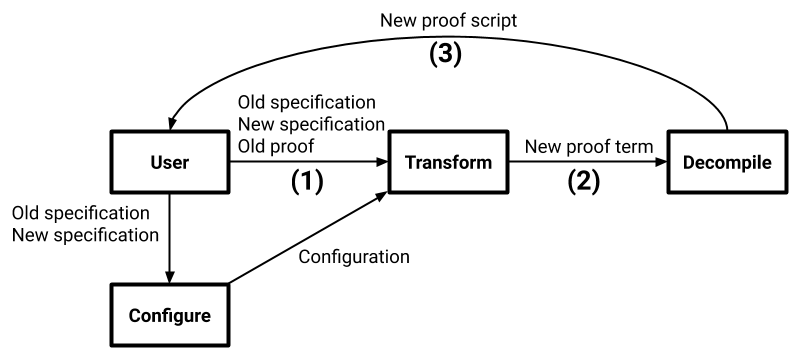
\includegraphics[width=\linewidth]{workflowa.png}
\end{minipage}
\hfill
\begin{minipage}{0.49\textwidth}
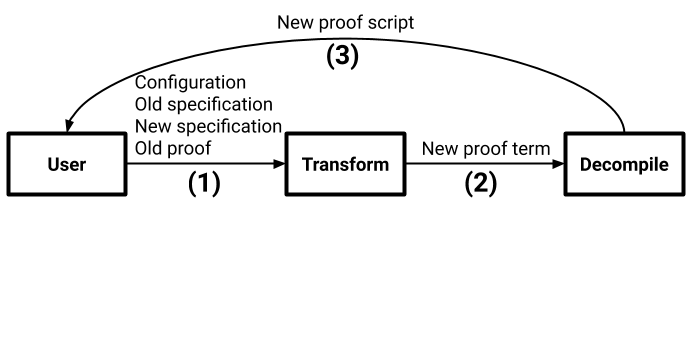
\includegraphics[width=\linewidth]{workflowb.png}
\end{minipage}
\caption{The two possible workflows for \toolname, using either automatic (left) or manual (right) configuration.}
\label{fig:system}
\end{figure}

The repair step works using a configurable program transformation.
This program transformation transforms the old proof term into a new proof term that refers to the new specification
(here, the theorem that refers to \lstinline{Coq.Init.Datatypes.list})
in place of the old specification (here, the theorem that refers to our updated \lstinline{list}),
and otherwise preserves the behavior of the old proof term.
The configuration instantiates the program transformation to a particular change in specification---it corresponds
to a particular relation between the old and new specificationss.
Figure~\ref{fig:system} shows how this comes together when the user invokes \toolname:

\begin{enumerate}
\item \toolname configures itself, either:
\begin{enumerate}
\item automatically (left), using \textbf{Configure} to discover the configuration, or
\item manually (right), by taking the configuration as an argument.
\end{enumerate}
\item The configured \textbf{Transform} transforms the old proof term into the new proof term.
\item \textbf{Decompile} produces a new proof script from the new proof term.
\end{enumerate}

Our example uses automatic configuration. When we run the \lstinline{Repair} command:

\begin{lstlisting}
Repair Coq.Init.Datatypes.list list in Coq.Init.Datatypes.rev_app_distr.
\end{lstlisting}
\textbf{Configure} invokes a special search procedure that automatically discovers that our new \lstinline{list}
is just our old \lstinline{list} with a single moved constructor.
The search procedure proves an equivalence between our old and new versions of lists,
then configures \textbf{Transform} using that equivalence and some additional information.
\textbf{Transform} then ports the proof term that inducted over our old \lstinline{list}
to instead induct over our new \lstinline{list}, and finally
\textbf{Decompile} produces the tactic script that we see.

While this is a simple refactoring, this same workflow can get us much more.
Section~\ref{sec:search} shows how we have used \toolname to support industrial integration with Coq,
write dependently-typed functions and proofs with little user effort,
port proofs between unary and binary natural numbers,
and support repair examples from benchmarks from real Coq proof engineers in the wild.


